\documentclass[a4paper,12pt]{article}
\usepackage{cmap}
\usepackage[utf8]{inputenc}
\usepackage[warn]{mathtext}
\usepackage{epsf,amsmath,amsfonts,amssymb,amsbsy}
\usepackage[mathscr]{eucal}
\usepackage[english, russian]{babel}
\author{Мещеряков Павел Б02-920}
\title{Отчёт о выполнении лабораторной работы 2.2.1}
\usepackage[left=2cm,right=2cm,top=2cm,bottom=2cm]{geometry}
\usepackage{graphicx}
\usepackage{indentfirst}
\graphicspath{{pictures2.2.1/}}
\DeclareGraphicsExtensions{.pdf,.png,.jpg}
\usepackage{pgfplots}
\usepackage{rotating}
\usepackage{pgfplotstable}
\usepackage{booktabs}
\usepackage{multirow}
\begin{document}
	\maketitle
	\begin{center}
		{\Large Определение теплоты испарения жидкости}
	\end{center}
\noindent \textbf{Цель работы:} \\
\indent 1)  регистрация  зависимости  концентрации   гелия в воздухе от времени с помощью датчиков теплопроводности при разных начальных давлениях смеси газов; 2) определение коэффициента диффузии по результатам измерений.\\
\noindent \textbf{В работе используются:} \\
\indent измерительная установка; форвакуумный насос; баллон с газом (гелий); манометр; источник питания; магазин сопротивлений; гальванометр; секундомер.

\section*{Теоретическое введение}
Рассмотрим процесс выравнивания концентрации. Пусть концентрации одного из компонентов смеси в сосудах $V_1$ и $V_2$ равны $n_1$ и
$n_2$. Плотность диффузионного потока любого компонента (т. е. количество вещества, проходящее в единицу времени через единичную поверхность) определяется законом Фика:
$$j=-D\frac{\partial n}{\partial x},$$ где $D$ — коэффициент взаимной диффузии газов, а $j$ - плотность потока частиц.

В нашем случае ввиду того что, а) объем соединительной трубки мал по сравнению с объемами сосудов, б) концентрацию газов внутри каждого сосуда можно считать постоянной по всему объему. Диффузионный поток в любом сечении трубки одинаков. Поэтому, $$J=-DS\frac{n_1-n_2}{l}.$$

Обозначим через $\Delta n_1$ и $\Delta n_2$ изменения концентрации в объемах
$V_1$ и $V_2$ за время $\Delta t$. Тогда $V_1 \Delta n_1$ равно изменению количества компонента в объеме $V_1$, а $V_2 \Delta n_2$ — изменению количества этого компонента в $V_2$. Из закона сохранения вещества следует, что $V_1n_1+V_2n_2 = const$, откуда $V_1 \Delta n_1 = -V_2\Delta n_2.$ Эти изменения происходят вследствие диффузии, поэтому: $$V_1\Delta n_1=-V_2\Delta n_2.$$

С другой стороны $V_1\Delta n_1=J\Delta t$ и $V_1\frac{dn_1}{dt}=-DS\frac{n_1-n_2}{l}.$ Аналогично $V_2\frac{dn_2}{dt}=DS\frac{n_1-n_2}{l}$

Тогда $$\frac{d(n_1-n_2)}{dt}=-\frac{n_1-n_2}{l} \frac{V_1+V_2}{V_1V_2}.$$

Проинтегрируем и получим, что $$n_1-n_2=(n_1-n_2)_0 e^{-t/\tau},$$ где $(n_1-
n_2)_0$ — разность концентраций в начальный момент времени, $$\tau=\frac{V_1V_2}{V_1+V_2}\frac{l}{SD}.$$

Для измерения концентраций в данной установке применяются датчики теплопроводности $Д_1$, $Д_2$ (см. рис. 1) используется зависимость теплопроводности газовой смеси от ее состава.
Для измерения разности концентраций газов используется мостовая схема (рис. 1). Здесь $Д_1$ и $Д_2$ — датчики теплопроводности, расположенные в сосудах $V_1$ и $V_2$. Сопротивления $R_1, R_2$ и $R$ служат для установки прибора на нуль (балансировка моста). В одну из диагоналей моста включен гальванометр, к другой подключается небольшое постоянное напряжение. Мост балансируется при заполнении сосудов (и датчиков) одной и той же смесью.

При заполнении сосудов смесями различного состава возникает «разбаланc» моста. При незначительном различии в составах смесей показания гальванометра, подсоединённого к диагонали моста, будут пропорциональны разности концентраций примеси. В процессе диффузии
разность концентраций убывает по экспоненте, и значит по тому же закону изменяются во времени показания гальванометра $$U=U_0 \exp(-t/\tau).$$
\section*{Эксперементальная установка}
Схема установки изображена на рис. 1. Там же показана схема электрических соединений и конструкция многоходового крана $K_6$

\begin{figure}[h]
	\center{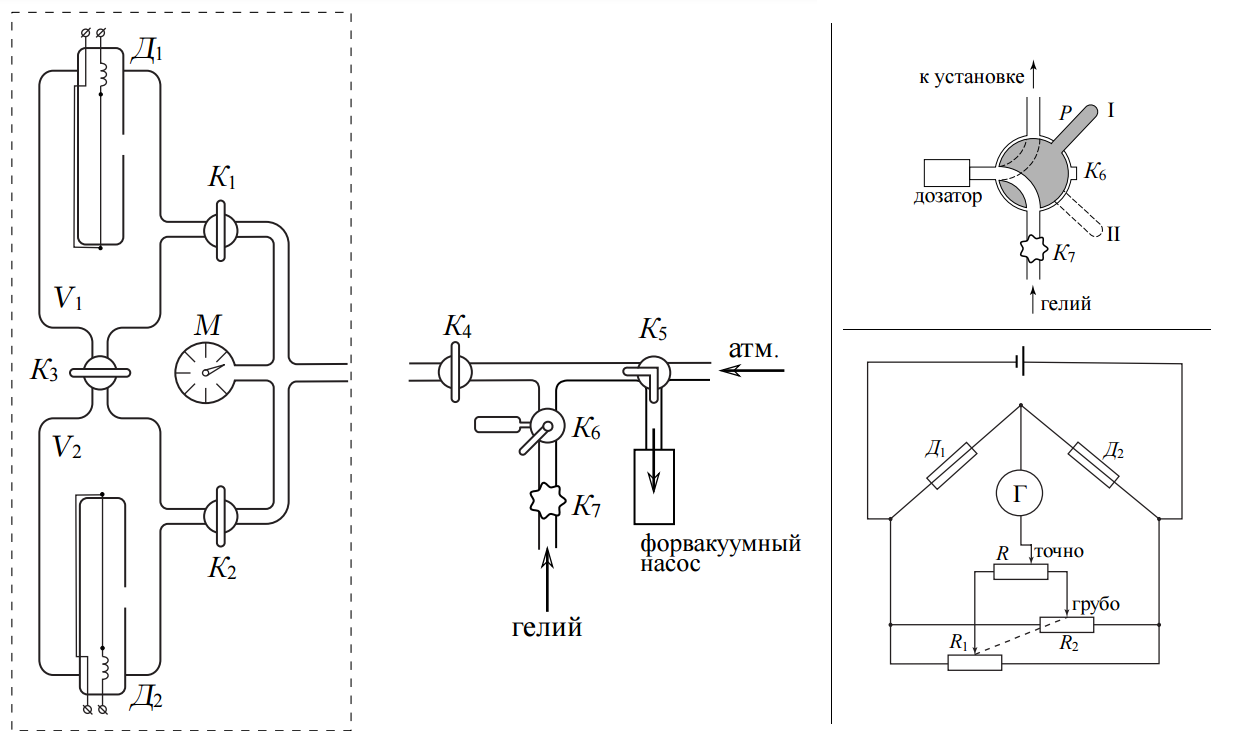
\includegraphics[scale=0.6]{lab_2_2_1_ust}}
	\caption{схема установки}
\end{figure}
Установка состоит из двух сосудов $V_1$ и $V_2$ соединенных краном $К_3$, форвакуумного насоса Ф.Н. с выключателем $Т$, манометра $M$ и системы напуска гелия, включающей в себя краны $К_6$ и $К_7$. Кран $К_5$ позволяет соединять форвакуумный насос либо с установкой, либо с атмосферой. Между форвакуумным насосом и краном $К_5$ вставлен предохранительный баллон П.Б., защищающий кран $К_5$ и установку при неправильной эксплуатации ее от попадания форвакуумного масла из насоса Ф.Н. Сосуды $V_1$ и $V_2$ и порознь и вместе можно соединять как с системой напуска гелия, так и с форвакуумным насосом. Для этого служат краны $К_1$, $К_2$, $К_4$ и $К_5$. Манометр  $M$
регистрирует давление газа, до которого заполняют тот или другой
сосуды.

Для сохранения гелия, а также для уменьшения неконтролированного попадания гелия в установку (по протечкам в кране $К_6$) между
трубопроводом подачи гелия и краном $К_6$ поставлен металлический
кран $К_7$. Его открывают только на время непосредственного заполнения установки гелием. Все остальное время он закрыт.

В силу того, что в сосуд требуется подавать малое давление гелия,
между кранами $К_7$ и $К_4$ стоит кран $К_6$, снабженный дозатором. Дозатор - это маленький объем, который заполняют до давления гелия в трубопроводе, а затем уже эту порцию гелия с помощью крана $К_6$ впускают в установку.

Описание схемы электрического соединения. $Д_1$ и $Д_2$ — сопротивления проволок датчиков парциального давления, которые составляют одно плечо моста. Второе плечо моста составляют сопро- тивления $r_1$, $R_1$ и $r_2$, $R_2$. $r_1 \ll R_1$, $r_2 \ll R_2$, $R_1$ и $R_2$ спаренные, их подвижные контакты находятся на общей оси. Оба они исполь- зуются для грубой регулировки моста. Точная балансировка моста выполняется потенциометром R. Последовательно с гальванометром $Г$, стоящим в диагонали моста, поставлен магазин сопротивлений $MR$. Когда мост балансируют, магазин сопротивлений выводят на ноль. В процессе же составления рабочей смеси в сосудах $V_1$ и $V_2$ мост разбалансирован. Чтобы не сжечь при этом гальванометр, магазин $MR$ ставят на максимальное сопротивление.

\section{Ход работы}
\begin{enumerate}
\item Включим питание электрической схемы установки рубильником $B$. Откроем краны $К_1$, $K_2$, $К_3$. Перепишем параметры установки: $$V_1 = V_2 = V = 800 \pm 5 \; см^{3}, \; \frac{L}{S} = 15.0 \pm 0.1 \;см^{-1}$$
Поскольку манометр измеряет разность давления внутри резервуаров с атмосферным в $\frac{кгс}{cм^2}$ необходимо записать показание манометра при полностью откачанном сосуде $P_0 = 98.0 \;\frac{кгс}{cм^2}$ (оно равно атмосферному) и в дальнейшем постоянно вычитать из него показания прибора, тем самым будет найдено давление внутри установки.
\item Очистим установку от всех газов, которые в ней есть. Для этого откроем кран $К_4$. Включим форвакуумный насос (Ф.Н.) выключателем $Т$, находящемся на насосе, и соединим насос с установкой, повернув ручку крана $К_5$ длинным концом рукоятки влево (на установку). Откачаем установку до давления $\approx 0.1 \; торр $, что достигается непрерывной работой насоса в течение 3–5 минут. Для прекращения откачки ручку крана $К_5$ поставим длинным концом вверх.
\item  Напустим в установку воздух до рабочего давления (вначале $P \approx 60 \; торр$), чтобы сбалансировать мост на рабочем давлении. Для этого рукоятку крана $К_5$ повернём из положения вправо (воздух поступает в насос) в положение влево (воздух из насоса поступает в установку). Эту операцию повторим несколько раз, пока не будет достигнуто нужное давление. Сбалансируем мост.
\item Заполним установку рабочей смесью согласно порядку предложенному в указании к работе: в сосуде $V_2$ должен быть воздух, а в сосуде $V_1$ — смесь воздуха, с гелием.

\item Проведём измерения. Для этого откроем кран $К_3$, включим компьютер
и затем скачаем из него данные показаний гальванометра с течением времени. Процесс измерений продолжим до тех пор, пока разность концентраций (показания гальванометра) не упадет на $40–50\%.$ Будем продолжать аналогичные измерения при различных значениях $P_{рабочее}$ в интервале $40–180 \; торр$. Данные представлены в таблице 1. Давления там приведены уже в торр.


\begin{sidewaystable}[]
\caption{Данные полученные с помощью компьютера}
%\begin{turn}{90}
	\begin{tabular}{|l|l|l|l|l|l|l|l|l|l|l|l|l|l|l|l|}
		\hline

		\multicolumn{16}{|c|}{$P, торр$}                                                                                                                                                        \\ \hline
		\multicolumn{4}{|c|}{60.00}                 & \multicolumn{4}{c|}{100.00}                 & \multicolumn{4}{c|}{140.00}                 & \multicolumn{4}{c|}{180.00}                 \\ \hline
		$t,c$    & $U,мв$ & $\ln{\frac{U}{U_0}}$ & $\sigma_{\ln{\frac{U}{U_0}}}$ & $t,c$    & $U,мв$ & $\ln{\frac{U}{U_0}}$ & $\sigma_{\ln{\frac{U}{U_0}}} $& $t,c$    & $U,мв$ & $\ln{\frac{U}{U_0}}$ & $\sigma_{\ln{\frac{U}{U_0}}}$ & $t,c$    & $U,мв$ & $\ln{\frac{U}{U_0}}$ & $\sigma_{\ln{\frac{U}{U_0}}}$ \\ 
		\hline
		0.00   & 9.24   & 0.00     & 0.008          & 0.00   & 18.25  & 0.00     & 0.004          & 0.00   & 16.46  & 0.00     & 0.004          & 0.00   & 17.22  & 0.00     & 0.004          \\ \hline
		19.98  & 8.98   & -0.03    & 0.008          & 31.90  & 17.72  & -0.03    & 0.004          & 41.81  & 15.98  & -0.03    & 0.004          & 34.91  & 16.83  & -0.02    & 0.004          \\ \hline
		41.98  & 8.68   & -0.06    & 0.008          & 63.90  & 17.16  & -0.06    & 0.004          & 83.81  & 15.46  & -0.06    & 0.004          & 69.91  & 16.46  & -0.04    & 0.004          \\ \hline
		61.98  & 8.41   & -0.09    & 0.008          & 95.90  & 16.62  & -0.09    & 0.004          & 125.81 & 14.97  & -0.09    & 0.005          & 104.91 & 16.11  & -0.07    & 0.004          \\ \hline
		83.98  & 8.13   & -0.13    & 0.008          & 127.90 & 16.10  & -0.12    & 0.004          & 167.81 & 14.51  & -0.13    & 0.005          & 139.91 & 15.78  & -0.09    & 0.004          \\ \hline
		103.98 & 7.89   & -0.16    & 0.008          & 159.90 & 15.61  & -0.16    & 0.004          & 209.81 & 14.07  & -0.16    & 0.005          & 174.91 & 15.46  & -0.11    & 0.004          \\ \hline
		125.98 & 7.63   & -0.19    & 0.009          & 191.90 & 15.14  & -0.19    & 0.004          & 251.81 & 13.65  & -0.19    & 0.005          & 209.91 & 15.16  & -0.13    & 0.004          \\ \hline
		145.98 & 7.40   & -0.22    & 0.009          & 223.90 & 14.69  & -0.22    & 0.004          & 293.81 & 13.24  & -0.22    & 0.005          & 244.91 & 14.86  & -0.15    & 0.004          \\ \hline
		167.98 & 7.15   & -0.26    & 0.009          & 255.90 & 14.25  & -0.25    & 0.004          & 335.81 & 12.85  & -0.25    & 0.005          & 279.91 & 14.58  & -0.17    & 0.004          \\ \hline
		187.98 & 6.94   & -0.29    & 0.009          & 287.90 & 13.84  & -0.28    & 0.005          & 377.81 & 12.48  & -0.28    & 0.005          & 314.91 & 14.30  & -0.19    & 0.005          \\ \hline
		209.98 & 6.72   & -0.32    & 0.009          & 319.90 & 13.43  & -0.31    & 0.005          & 419.81 & 12.12  & -0.31    & 0.005          & 349.91 & 14.03  & -0.20    & 0.005          \\ \hline
		229.98 & 6.52   & -0.35    & 0.009          & 351.90 & 13.04  & -0.34    & 0.005          & 461.81 & 11.77  & -0.34    & 0.005          & 384.91 & 13.78  & -0.22    & 0.005          \\ \hline
		251.98 & 6.31   & -0.38    & 0.010          & 383.90 & 12.67  & -0.36    & 0.005          & 503.81 & 11.44  & -0.36    & 0.005          & 419.91 & 13.52  & -0.24    & 0.005          \\ \hline
		271.98 & 6.13   & -0.41    & 0.010          & 415.90 & 12.30  & -0.39    & 0.005          & 545.81 & 11.11  & -0.39    & 0.005          & 454.91 & 13.28  & -0.26    & 0.005          \\ \hline
		293.98 & 5.93   & -0.44    & 0.010          & 447.90 & 11.96  & -0.42    & 0.005          & 587.81 & 10.81  & -0.42    & 0.006          & 489.91 & 13.04  & -0.28    & 0.005          \\ \hline
		313.98 & 5.76   & -0.47    & 0.010          & 479.90 & 11.62  & -0.45    & 0.005          & 629.81 & 10.51  & -0.45    & 0.006          & 524.91 & 12.81  & -0.30    & 0.005          \\ \hline
		335.98 & 5.58   & -0.50    & 0.010          & 511.90 & 11.29  & -0.48    & 0.005          & 671.81 & 10.22  & -0.48    & 0.006          & 559.91 & 12.58  & -0.31    & 0.005          \\ \hline
		355.98 & 5.43   & -0.53    & 0.011          & 543.90 & 10.98  & -0.51    & 0.005          & 713.81 & 9.94   & -0.50    & 0.006          & 594.91 & 12.36  & -0.33    & 0.005          \\ \hline
		377.98 & 5.26   & -0.56    & 0.011          & 575.90 & 10.67  & -0.54    & 0.005          & 755.81 & 9.67   & -0.53    & 0.006          & 629.91 & 12.15  & -0.35    & 0.005          \\ \hline
		397.98 & 5.11   & -0.59    & 0.011          & 607.90 & 10.38  & -0.56    & 0.006          & 797.81 & 9.41   & -0.56    & 0.006          & 664.91 & 11.94  & -0.37    & 0.005          \\ \hline
		419.98 & 4.95   & -0.62    & 0.011          & 639.90 & 10.10  & -0.59    & 0.006          & 839.81 & 9.17   & -0.59    & 0.006          & 699.91 & 11.74  & -0.38    & 0.005          \\ \hline
		439.98 & 4.81   & -0.65    & 0.012          & 671.90 & 9.82   & -0.62    & 0.006          & 881.81 & 8.92   & -0.61    & 0.006          & 734.91 & 11.53  & -0.40    & 0.005          \\ \hline
		461.98 & 4.66   & -0.68    & 0.012          & 703.90 & 9.55   & -0.65    & 0.006          & 923.81 & 8.68   & -0.64    & 0.007          & 769.91 & 11.34  & -0.42    & 0.005          \\ \hline
		481.98 & 4.53   & -0.71    & 0.012          & 735.90 & 9.30   & -0.67    & 0.006          & 957.81 & 8.49   & -0.66    & 0.007          & 804.91 & 11.14  & -0.44    & 0.005          \\ \hline
	\end{tabular}
%\end{turn}
\end{sidewaystable}


\item Для каждого из давлений построим графики, откладывая по
оси абсцисс время, а по оси ординат - логарифм от показаний гальванометра. Видим, что теоретическая зависимость $U = U_0 \cdot e^{\frac{-t}{\tau}}$ подтверждается эксперементально.
\begin{center}
\begin{figure}[h!]
\begin{tikzpicture}[scale = 1.5]
\begin{axis}[
legend cell align={left},
axis x line=left,
axis y line=left,
legend style={at={(1,0.377)}},
ylabel= {$-\ln{\frac{U}{U_0}}$},
xlabel = {$ t,c $},
xmin=0, xmax=950,
ymin=0, ymax=0.8,
ymajorgrids = true,
xmajorgrids = true,
yminorgrids = true,
xminorgrids = true,
minor tick num = 4
]


\addplot +[only marks] 
plot table [		    	    	    	
x=t1, 
y=-U1]
{data_1.txt};


\addplot +[only marks] 
plot table [		    	    	    	
x=t2, 
y=-U2]
{data_2.txt};


\addplot +[only marks] 
plot table [		    	    	    	
x=t3, 
y=-U3]
{data_3.txt};


\addplot +[only marks] 
plot table [		    	    	    	
x=t4, 
y=-U4]
{data_4.txt};
\addplot[blue, domain=0:550]{+0.00424 +0.001479865*x};
\addplot[domain=0:1000]{+0.007604811 +0.000917233*x};
\addplot[domain=0:1000]{+0.010858935 +0.000689002*x};
\addplot[domain=0:1000]{+0.011878708 +0.000534871*x};
	\legend{
	$P = 60 \;торр$,$P = 100 \;торр$,$P = 140 \;торр$,$P = 180 \;торр$
};
\end{axis}
\end{tikzpicture}
\caption{График зависимости $-\ln{\frac{U}{U_0}}(t)$}
\end{figure}
\end{center}
%Запишу уравнения фитирующих прямых, параметры которых получены с помощью МНК:
\begin{center}
\begin{table}[h!]
\caption{Уравнения фитирующих прямых}
	\begin{tabular}{@{}|l|l|l|l|l|l|@{}}
		\toprule
		\multirow{4}{*}{P,торр} & 60  & \multicolumn{4}{l|}{$\ln{\frac{U}{U_0}} =-(42 \pm 16)\cdot 10^{-4} -(1480 \pm 5)\cdot 10^{-6} \;t$} \\ \cmidrule(l){2-6} 
		& 100 & \multicolumn{4}{l|}{$\ln{\frac{U}{U_0}} =-(76 \pm 20)\cdot 10^{-4} -(917 \pm 5)\cdot 10^{-6} \; t$} \\ \cmidrule(l){2-6} 
		& 140 & \multicolumn{4}{l|}{$\ln{\frac{U}{U_0}} =-(109 \pm 26)\cdot 10^{-4} -(689 \pm 4)\cdot 10^{-6} \;t$} \\ \cmidrule(l){2-6} 
		& 180 & \multicolumn{4}{l|}{$\ln{\frac{U}{U_0}} =-(119 \pm 22)\cdot 10^{-4} -(535 \pm 4)\cdot 10^{-6} \; t$} \\ \bottomrule
	\end{tabular}
\end{table}
\end{center}
По угловым коэффициентам экспериментальных прямых и известным параметрам установки рассчитаем коэффициенты взаимной диффузии и их погрешности при выбранных давлениях по формулам: $$D =  \frac{1}{2} kV \frac{L}{S}, \; \sigma_D = D \sqrt{\big(\frac{\sigma_k}{k}\big)^2 + \big(\frac{3\sigma_V }{2V}\big)^2 + \big(\frac{\sigma_{L/S}}{L/S}\big)^2},$$ где $k$ - коэффициенты наклонов прямых. Данные представлены в таблице 3.
 
 \begin{table}[!htb]
 	\centering
 	\begin{minipage}{0.45\linewidth}
 		\centering
 	\caption{}
 	\begin{tabular}{|l|l|l|}
 		\hline
 		\label{tb1}	
 		$P, торр$ & $D, \frac{см^2}{c}$ & $\sigma_D, \frac{см^2}{c}$ \\ \hline
 		60 &  8.88& 0.18 \\ 
 		\hline
 		100 & 5.50  & 0.11 \\ 
 		\hline
 		140 & 4.13 & 0.09 \\ 
 		\hline
 		180& 3.21 & 0.07 \\ 
 		\hline
 	\end{tabular}
\end{minipage}
\begin{minipage}{0.45\linewidth}
	\centering
	\caption{}
	\begin{tabular}{|c|c|c|}
		\hline
		\label{tb1}
		
		$\frac{1}{P} , торр^{-1}\cdot 10^{-3} $ & $\sigma_{\frac{1}{P}} ,\;торр^{-1}\cdot 10^{-3}$ & $D, \frac{см^2}{c} $\\ \hline
		16.67 & 2 & 8.88\\ 
		\hline
		10.00 & 0.8 &5.50 \\ 
		\hline
		7.14 & 0.4 &4.13 \\ 
		\hline
		5.56& 0.2 &3.21 \\ 
		\hline
	
	\end{tabular}
\end{minipage}
\end{table}

\item Построим график зависимости коэффициента диффузии от давления в координатах $D, \; \frac{1}{P}.$ Погрешность расчитывается по формуле $\sigma{_\frac{1}{P}} = \frac{\sigma_P}{P^2}$, где $\sigma_P = 7.4 \; {торр}$. Рассчитаем величину коэффициента диффузии при атмосферном давлении. Для этого экстраполируем зависимость $D(\frac{1}{P})$ и посмотрим через какую точку проходит наша прямая. Итак, $$D_{атм} =0.68 \pm 0.06  \; \frac{cм^2}{c}.$$ Погрешность $D_{атм}$ была оценена с помошью экстраполяции крайних уравнений прямых. Табличное значение для этого коэффициента $$D_{табл} = 0.57\;\frac{cм^2}{c}.$$


\begin{center}
\begin{figure}[h!]
\begin{tikzpicture}[scale = 1.5]
\begin{axis}[
axis lines = left,
legend style={at={(1,0.21)}},
ylabel = {$D,\frac{cм^2}{c}$},
xlabel = {$ \frac{1}{P} ,  {торр}^{-1} \cdot 10^{-3}$},
minor grid style={black, line width=0.05pt},
major grid style={solid,black, line width=0.3pt},
xmin=0, xmax=20,
ymin=0, ymax=10,
ymajorgrids = true,
xmajorgrids = true,
yminorgrids = true,
xminorgrids = true,
minor tick num = 4
]
\addplot+[only marks ] plot[error bars/.cd, x dir=both, x explicit]
coordinates {
	(16.67,8.88) +-(2,2) 
	(10.0,5.5) +-(0.8,0.8)
	(7.34, 4.13) +-(0.4,0.4)
	(5.76, 3.21)+-(0.2,0.2)
};
\addplot+[red,only marks ] plot[error bars/.cd, y dir=both, y explicit]
coordinates {
	(1.3158,0.74)
};
%\addplot[blue, domain=0:20]{0.448  + 0.5062*x};
\addplot[blue, domain=0:20]{0.0  + 0.54153*x};
\legend{
	$D = (514 \pm 47) \frac{1}{P}$,$D_{атм}$
};

\end{axis}
\end{tikzpicture}
\caption{График зависимости $D(\frac{1}{P}$)}
\end{figure}
\end{center}


\item Оценим по полученным результатам длину свободного пробега и размер молекулы.  Для этого воспользуемся следующими формулами. $$D = \frac{1}{3} \lambda \langle v \rangle,\; где \langle v \rangle = \sqrt{\frac{8RT}{\pi \mu}}, \; \Pi \approx \frac{kT}{\sqrt{2}\lambda P},$$ где $\Pi$ - площадь эффективного сечения частиц, $r \approx \frac{1}{2}\sqrt{\frac{\Pi}{\pi}}$.

Итак, $$\lambda \approx 1.6 \cdot 10^{-7} \; м, \; \Pi \approx 1.8\cdot 10^{-19} \; м^2, \; r \approx 1.2 \cdot 10^{-10}\; м.$$ Табличное значение для размера молекулы $r = 1.0 \cdot 10^{-10}\; м.$

\section{Вывод}
В данной работе было проверено, что закон $U = U_0 \cdot e^{\frac{-t}{\tau}}$ выполняется с высокой точностью.

Так же в работе было найдено значение коэффициента диффузии гелия в воздухе, а так же оценены длина свободного пробега и размер молекулы гелия. К сожалению, результат не сошёлся с табличным. Этому есть несколько разумных объяснений. Вероятно, были совершены ошибки на этапе заготовки смесей газов в сосудах (погрешности определения давлений) и ошибки экспериментатора. А так же есть подозрение, что газ, который в работе назывался гелием, на самом деле был разбавленным. Так же не стоит забывать о том, что численный множитель $\frac{1}{3}$ в формуле для длины свободного пробега, является на самом деле данью традиции, поэтому на ювелирную точность определения параметров в последнем пункте претендовать не стоит. В любом случае методика данной работы позволяет с достаточной точностью получить приблизительное значение коэффициента диффузии и позволяет оценить такие важные физические величины, как длина свободного пробега и размер молекулы газа.

\end{enumerate}
\end{document}